\documentclass[a4paper]{article}
\usepackage{amsmath}
\usepackage{amsfonts}
\usepackage{amsthm}
\usepackage{amssymb}
\usepackage[english]{babel}
\usepackage{float}
\usepackage{graphicx}
\usepackage{hyperref}
\usepackage[utf8]{inputenc}
\usepackage{listings}
\usepackage{xcolor}
%% \usepackage{subfigure}
\usepackage{pdfpages}
\usepackage{graphicx}
\usepackage{subcaption}
\usepackage{stmaryrd}
\usepackage{a4wide}

\lstset{
  frame=tb,
  language=Python,
  aboveskip=3mm,
  belowskip=3mm,
  showstringspaces=false,
  formfeed=newpage,
  tabsize=4,
  comment=[l]{\#},
  breaklines=true,
  basicstyle=\small
}

\newcommand{\prob}[1]{\mathbb{P}\left(#1\right)}
\newcommand{\expect}[1]{\mathbb{E}\left(#1\right)}
\newcommand{\avg}[1]{\sum_{i=1}^{#1}X_i}
%% \newcommand{\dotp}[2]{\langle #1 + #2 \rangle}
%% \newcommand{\dotp}[2]{\ensuremath{\frac{#1}{#2}}}
\newcommand{\dotpr}[2]{\langle #1,\; #2 \rangle}
\newcommand{\norm}[1]{\left\lVert#1\right\rVert}
\newcommand*{\QEDA}{\hfill\ensuremath{\blacksquare}}%

\title{\vspace{-5cm}ATML Home Assignment 3}
\author{Dmitry Serykh (qwl888)}

\begin{document}
\maketitle
\section{Introduction}
In this assignment, I have attempted to reproduce the second experiment from
Thiemann et al for the Ionosphere dataset. I based a portion of my implementation
(including the calculation Jaakkola's heuristic) on my own solution to a similar
exercise from the DIKU ML course that I took last year. The source code for my
implementation can be found in file \texttt{experiment.py} in
\textbf{handin.zip}.


\section{Practical Information}
I used \emph{python}, \emph{numpy} and SVM solver
from the \emph{sklearn} package. The experiment were ran on my laptop, running
Linux and with following hardware specifications:
\begin{verbatim}
 CPU: Intel Core i7-3520M @ 4x 3.6GHz
 RAM: 7682MiB
\end{verbatim}

\section{Theory}
I used the slightly tighter version of PAC-Bayes-kl inequality, as described in
the paper:
\[
\mathrm{kl}\left(\mathbb{E}_{\rho}[\hat{L}(h, S)] \|
\mathbb{E}_{\rho}[L(h)]\right) \leq \frac{\mathrm{KL}(\rho \| \pi)+\ln \frac{2
    \sqrt{n-r}}{\delta}}{n-r}
\]
which holds with probability $1 - \delta$ for all distributions $\rho \in
\mathcal{H}$. I used the numerical inversion of the kl divergence from the first
assignment in order to bound the test loss of the PAC-Bayesian aggregation model.\\\\
I used a following numerically stable
update rule for $\rho$, as suggested in the assignment text.
\[
\rho(h) = 
\frac{\left.\pi(h) e^{-\lambda(n-r)\left(\hat{L}^{\mathrm{val}(h, S)}-\hat{L}_{\mathrm{min}}^{\mathrm{val}}\right.}\right)}{\sum_{h^{\prime}} \pi\left(h^{\prime}\right) e^{-\lambda(n-r)\left(\hat{L}^{\mathrm{val}}\left(h^{\prime}, S\right)-\hat{L}_{\mathrm{min}}^{\mathrm{val}}\right)}}
\]
For the $\lambda$ update, I used the formula from the paper:
\[
\lambda=\frac{2}{\sqrt{\frac{2(n-r) \mathbb{E}_{\rho}[\hat{L}(h, S)]}{\left(\mathrm{KL}(\rho \| \pi)+\ln \frac{2 \sqrt{(n-r)}}{\delta}\right)}+1+1}}
\]
I used uniform distribution for the value of $\pi(h)$ and the initial value of
$\rho(h)$. I chose 1 to be the initial value of $\lambda$ and set $\delta =
0.05$, as in the paper. I also used weighted majority vote aggregation (the
discrete case), as described in the lecture notes, by calculating.
\[
\operatorname{sign}\left(\sum_{h \in \mathcal{H}} \rho(h) h(X)\right)
\]
where I chose $\operatorname{sign}(0)=1$\\\\

\section{Results}
I decided not to repeat the ``sin'' that was committed in the original paper and
repeated the whole experiment 25 times and find the average of the gathered
results. Moreover, I calculated the standard deviation of the test losses and
runtimes for both methods:

\begin{verbatim}
Standard deviations:
PAC-Bayesian loss: 0.0982
CV loss: 0.0147
PAC-Bayesian time: 0.0575
CV time: 0.0441
\end{verbatim}
The resulting plot of average test losses of PAC-Bayesian aggregation and RBF
kernel SVM tuned by cross-validation, running times ($t_m$ and $t_{CV}$) and
bound can be seen on Figure \ref{plt1}.\\\\
The test loss of the PAC-Bayesian aggregation decreases with increasing
$m$, and it nears the test loss of the baseline model when the value of $m$
approaches $n$. \\
Furthermore, the runtime for the PAC-Bayesian aggregation method
is much better than the baseline model. The runtime grows linearly with the
value of $m$ (which looks exponential on the plot due to logarithmic scale of
x-axis), which is akin to the results in the paper. \\
Lastly, as one would expect, there are discrepancies between my plot and the
original due to nondeterministic nature of the algorithm. I would, however, argue
that I managed to achieve results, similar to the original experiment, and
the main data trends of the original are captured on my plot.

\newpage
\vspace*{\fill}
\begin{figure}[H]
  \centering
  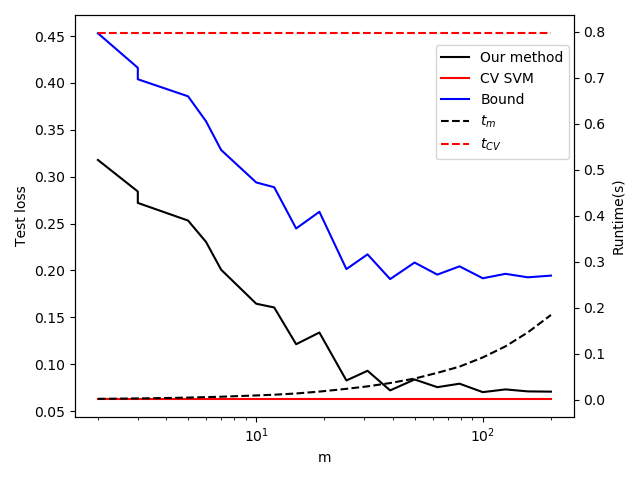
\includegraphics[width=\textwidth]{code/plt_avg25_1}
  \caption{Comparison of PAC-Bayesian aggregation with RBF kernel SVM
    tuned by cross-validation for the Ionosphere dataset. Averaged over 25 experiments, $n=200$, $r=35$}
  \label{plt1}
\end{figure}
\vspace*{\fill}

\end{document}

%% \begin{figure}
%%   \centering
%%   \begin{subfigure}[b]{\textwidth}
%%     \centering
%%     \includegraphics[scale=0.8]{handin/plt51}
%%     \caption{Classification of the training set}
%%   \end{subfigure}
%%   \begin{subfigure}[b]{\textwidth}
%%     \centering
%%     \includegraphics[scale=0.8]{handin/plt52}
%%     \caption{Classification of the test set}
%%   \end{subfigure}
%%   \caption{Exercise 5: Logistic Regression Applied to the Datasets}
%%   \label{plt5}
%% \end{figure}

%% \begin{lstlisting}[caption="Calculation of g"]
%% def calc_g(Xs, y, w):
%%     N = np.shape(Xs)[0]
%%     # use matrix X of xs instead of for-loop = much faster
%%     X = np.c_[Xs, np.ones(N)]
%%     num = y.T * X
%%     denum = 1 + np.exp(y * (w @ X.T))
%%     M = num.T/denum
%%     # return mean of each row
%%     return (-1 * np.mean(M, axis=1))
%% \end{lstlisting}
